\documentclass{beamer}
\usepackage[utf8]{inputenc}
\usepackage{listings}
\usepackage{graphicx}
\usepackage{xcolor}
\usepackage{hyperref}
\usepackage{graphicx}
\usepackage{float}
\usepackage{amsmath}
\usepackage{relsize}
\usepackage{listings}
% \usepackage{enumitem}
\usepackage{fancyhdr}
\usepackage{booktabs}
\usepackage{multirow}
\usepackage{tabularx}
\usepackage{multirow}
\colorlet{lightgrey}{lightgray}
\usepackage{colortbl}
\usepackage[bibstyle=authoryear, style=numeric, citestyle=numeric-comp, backend=bibtex]{biblatex}
\bibliography{bibliography/krr,bibliography/procs,local}
\usetheme{Antibes}
\setbeamertemplate{footline}[frame number]
\title{Generate, filter and merge single agent paths for Multi Agent Pathfinding using Answer Set Programming}
\author{Aurélien SIMON}
\begin{document}

\lstdefinestyle{mystyle}{
    basicstyle=\tiny,
    % frame=single,
    breaklines,
    columns=fullflexible,
    breakindent=1.2em,
    breakatwhitespace,
    numbers=left, 
    escapechar=|
}


\lstdefinestyle{small}{
    basicstyle=\small,
    % frame=single,
    breaklines,
    columns=fullflexible,
    breakindent=1.2em,
    breakatwhitespace,
    numbers=left, 
    escapechar=|
}



\begin{frame}
\titlepage
\end{frame}


\newcommand\widthimg{8cm}

\begin{frame}{Table of Content}\
    \tiny
    \tableofcontents
\end{frame} 


\section{Introduction \& Background}
\subsection{What is MAPF?}
\begin{frame}
    \textbf{What is Multi Agent PathFinding?} \\[1cm]

    \(\blacktriangleright \) Multi-Agent Pathfinding (MAPF) involves planning collision-free paths for multiple agents in a shared environment.

    \(\blacktriangleright \) Various application : warehouse management~\cite{wurman2008coordinating}, video games~\cite{ma2017feasibility}, routing, planning, robotics~\cite{veloso2015cobots}\dots


\end{frame}

\begin{frame}{An example}
    
    \begin{figure}[H]
        \centering
        \caption{Example of Multi agent Pathfinding}
        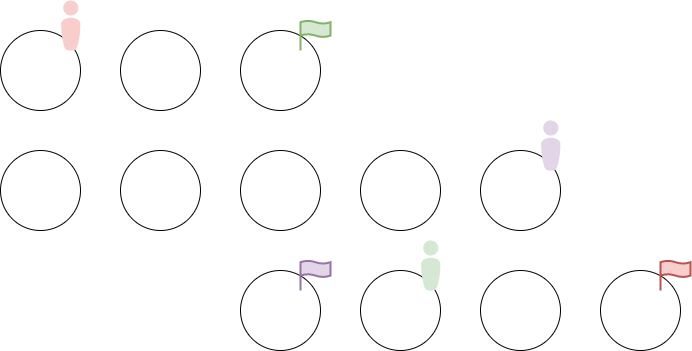
\includegraphics[width=\widthimg]{img/MAPF_example_1.drawio.png}
    \end{figure}

\end{frame}


\begin{frame}{An example}
    
    \begin{figure}[H]
        \centering
        \caption{Example of Multi agent Pathfinding}
        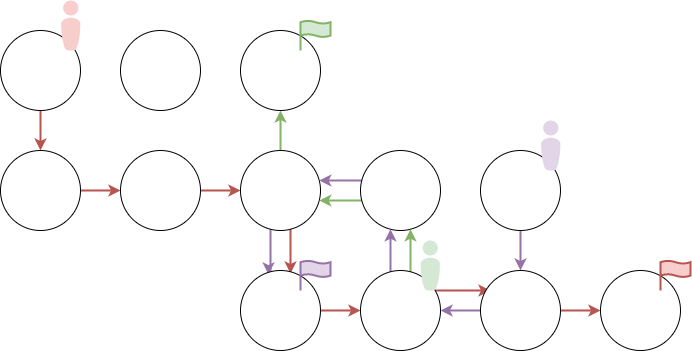
\includegraphics[width=\widthimg]{img/MAPF_example_2.drawio.png}
    \end{figure}

\end{frame}


\begin{frame}{Settings}
    MAPF is defined on a graph.
    
    \begin{block}{Nomenclature}
        \begin{itemize}
            \item The output is a plan \(\Pi\)
            \item \(\Pi\) is a collection of \(\pi\)
        \end{itemize}
    \end{block}
    
    
    \begin{figure}[H]
        \centering
        \caption{Considered conflicts}
        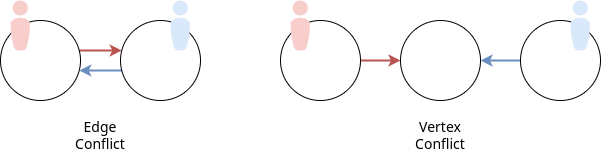
\includegraphics[width=\widthimg]{img/conflict_type.drawio.png}
    \end{figure}


\end{frame}



\subsection{Plan Merging: Motivation, Principle \& Overview}

\begin{frame}{Plan Merging: Motivation, Principle \& Overview}


    \textbf{Principle}
    \begin{itemize}
        \item From path(S) computed without considering conflict
        \item Try to find a conflict free plan out of the previously computed paths
    \end{itemize}


    \textbf{Motivation}
    \begin{itemize}
        \item Computing multiple individual path(s) is not expensive
        \item + Combining them is still faster 
    \end{itemize}


    \textbf{Overview}
    \begin{figure}[H]
        \centering
        \caption{Overview of the process}
        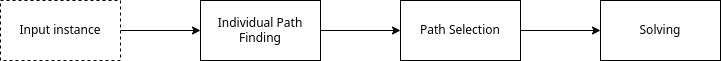
\includegraphics[width=\widthimg]{img/overview.drawio.png}
    \end{figure}
\end{frame}


\section{Individual Path Finding}
\begin{frame}{Individual Path Finding}
    What is Individual Path finding?
    \begin{itemize}
        \item Creating \(n\) paths for each agents
        \item Creating \textbf{different kind of paths}
        \item Paths created do not consider collision with other paths
    \end{itemize}
    \begin{itemize}
        \item For each agent \(a\), we have \(\gamma_a\) = \(\{\pi_0,\dots,\pi_n\}\)
        \begin{itemize}
            \item \(\gamma\) is a set of paths
        \end{itemize}
        \item \(\tau\) representing the output of IPF 
        \begin{itemize}
            \item \(\tau = \{\gamma_a, \gamma_{a'}, ...\}\) is a set of set of paths
        \end{itemize}
    \end{itemize}
\end{frame}


\begin{frame}{IPF output example}
    \begin{figure}[H]
        \centering
        \caption{Example of a \(\tau = \{\gamma_r, \gamma_b, \gamma_g\}\)}\label{fig:ipf_example}
        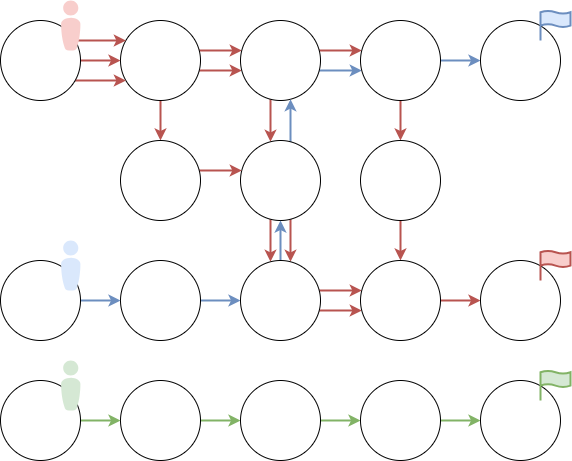
\includegraphics[width=7cm]{img/ipf_example.drawio.png}
    \end{figure}
\end{frame}



\subsection{IPF Computation}

\begin{frame}{Base IPF Computation}
    Principle of Base IPF computation
    \begin{figure}[H]
        \centering
        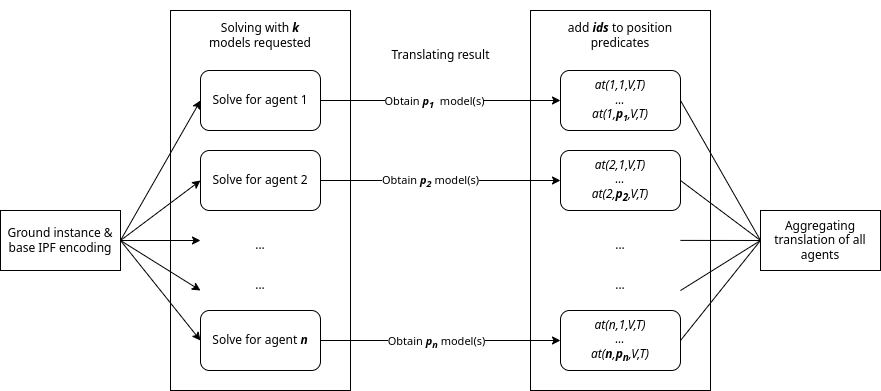
\includegraphics[width=11cm]{img/flowchart_ipf_computation.drawio.png}
    \end{figure}
\end{frame}

\section{Path Selection}
\begin{frame}{Path Selection}
    Path Selection aims to create an ``interesting'' subcomponent \(\tau'\) of \(\tau\). 

    \begin{figure}[H]
        \centering
        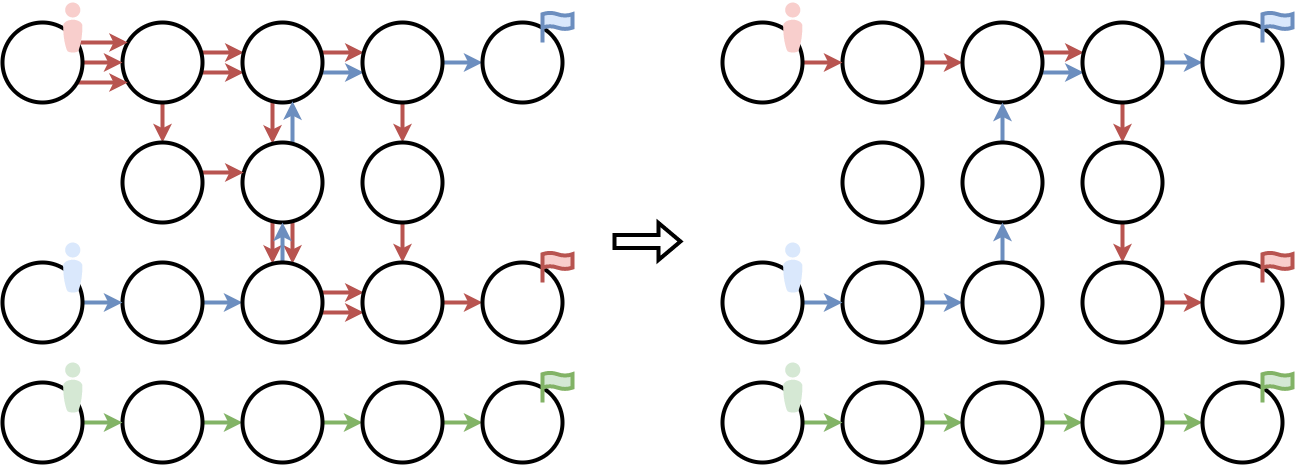
\includegraphics[width=11cm]{img/pm_example_intro.png}
    \end{figure}

\end{frame}


\subsection{Path Elimination}
\begin{frame}{Path Elimination}
    \textbf{  Path Elimination} is the process of the removing paths that exhibit potential issues. 
    
    \begin{block}{Why not find brute force a conflict-free set of paths directly?}
        \(\text{    }\blacktriangleright\) Slow with a lot of agents and paths, we need some preliminary process first
    \end{block}

    Two ways:
    \begin{itemize}
        \item \textbf{Based on heatmaps}
        \item Based on potential conflict
    \end{itemize}

\end{frame}


\subsection{Individual Heatmap}
\begin{frame}[fragile]{Individual Heatmap}
    Individual Heatmap is about projecting likelihood of presence of an agent on vertices
at each step.

    \[
        \phi(\gamma,v,t) = \frac{| \{\pi|\pi \in \gamma,\pi(t) = v\}|}{|\gamma|}
    \]


\end{frame}

\begin{frame}{Individual Heatmap example 1/5}

    \begin{figure}[H]
        \centering
        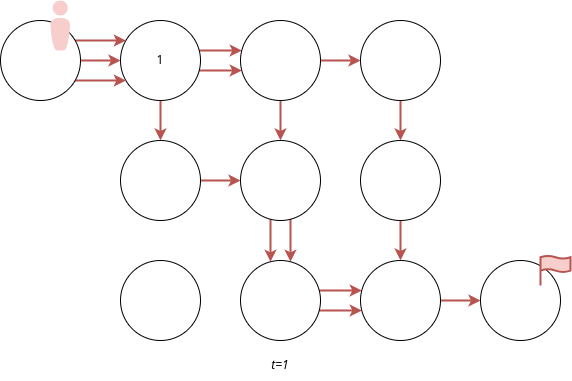
\includegraphics[width=9cm]{img/individual_heatmap_p1.drawio.png}
    \end{figure}
\end{frame}

\begin{frame}{Individual Heatmap example 2/5}
    \begin{figure}[H]
        \centering
        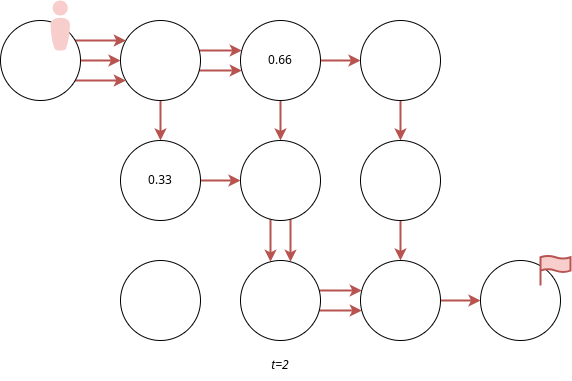
\includegraphics[width=9cm]{img/individual_heatmap_p2.drawio.png}
    \end{figure}
\end{frame}


\begin{frame}{Individual Heatmap example 3/5}
    \begin{figure}[H]
        \centering
        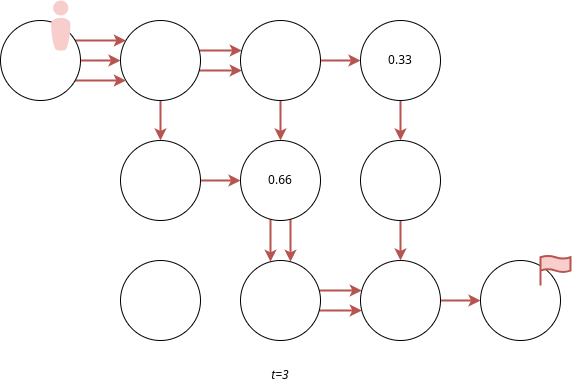
\includegraphics[width=9cm]{img/individual_heatmap_p3.drawio.png}
    \end{figure}
\end{frame}

\begin{frame}{Individual Heatmap example 4/5}
    \begin{figure}[H]
        \centering
        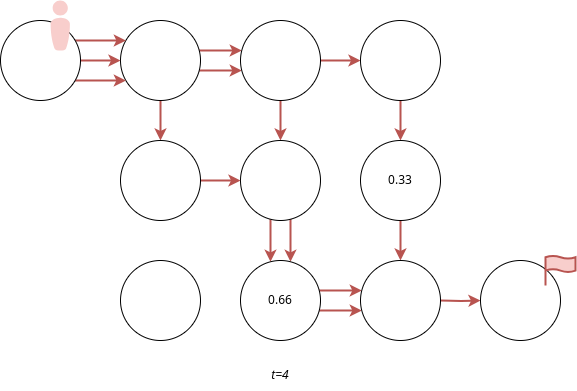
\includegraphics[width=9cm]{img/individual_heatmap_p4.drawio.png}
    \end{figure}
\end{frame}

\begin{frame}{Individual Heatmap example 5/5}
    \begin{figure}[H]
        \centering
        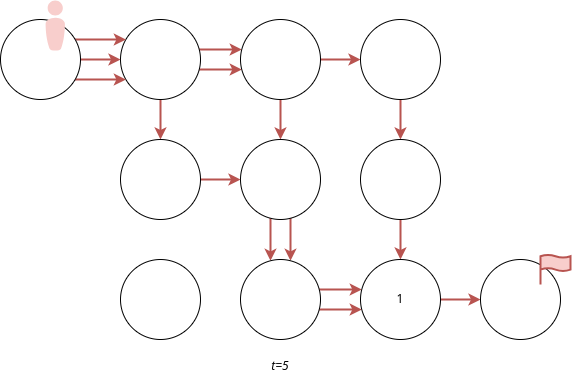
\includegraphics[width=9cm]{img/individual_heatmap_p5.drawio.png}
    \end{figure}
\end{frame}

\subsection{Global Heatmap}

\begin{frame}{Global Geatmap}
    We derive a \textbf{Global Heatmap} (GH) through the aggregation of all Individual Heatmaps
    \[
        \Phi(\tau,v,t) = \frac{ \sum_{\gamma \in \tau}\phi(\gamma,v,t)}{|\tau|}
    \]

    Global Heatmap do not represent a direct indicator of the likelihood of presence but instead an indicator of ``usage of vertices'' by multiple agents
\end{frame}


\begin{frame}{Global Heatmap example 1/5}
    \begin{figure}[H]
        \centering
        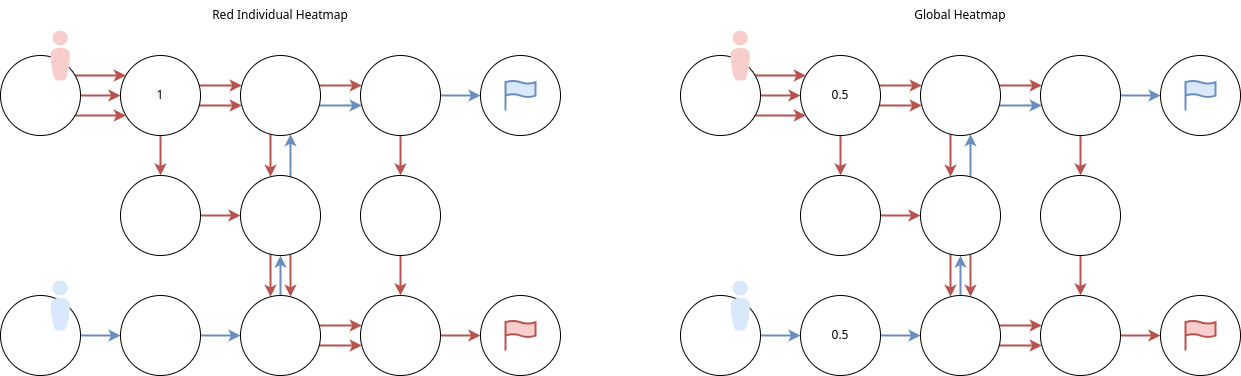
\includegraphics[width=11cm]{img/global_heatmap_p1.drawio.png}
    \end{figure}
\end{frame}


\begin{frame}{Global Heatmap example 2/5}
    \begin{figure}[H]
        \centering
        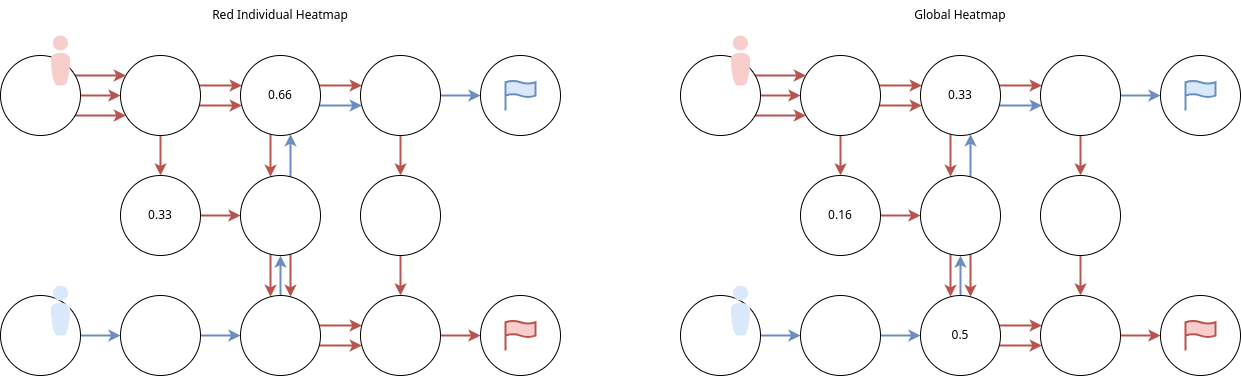
\includegraphics[width=11cm]{img/global_heatmap_p2.drawio.png}
    \end{figure}
\end{frame}



\begin{frame}{Global Heatmap example 3/5}
    \begin{figure}[H]
        \centering
        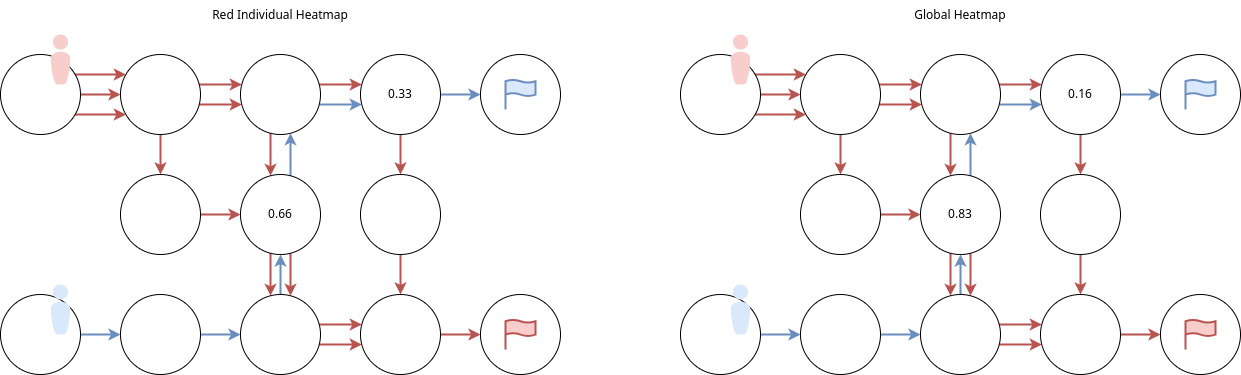
\includegraphics[width=11cm]{img/global_heatmap_p3.drawio.png}
    \end{figure}
\end{frame}


\begin{frame}{Global Heatmap example 4/5}
    \begin{figure}[H]
        \centering
        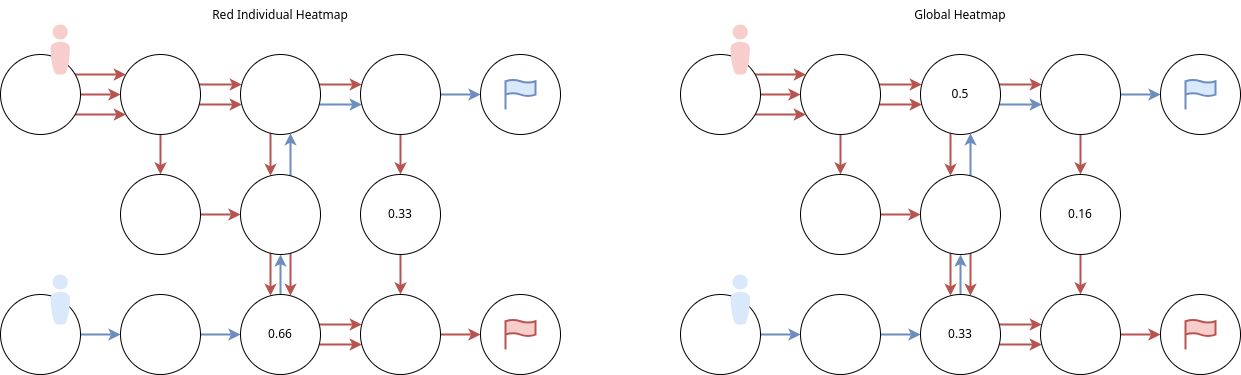
\includegraphics[width=11cm]{img/global_heatmap_p4.drawio.png}
    \end{figure}
\end{frame}


\begin{frame}{Global Heatmap example 5/5}
    \begin{figure}[H]
        \centering
        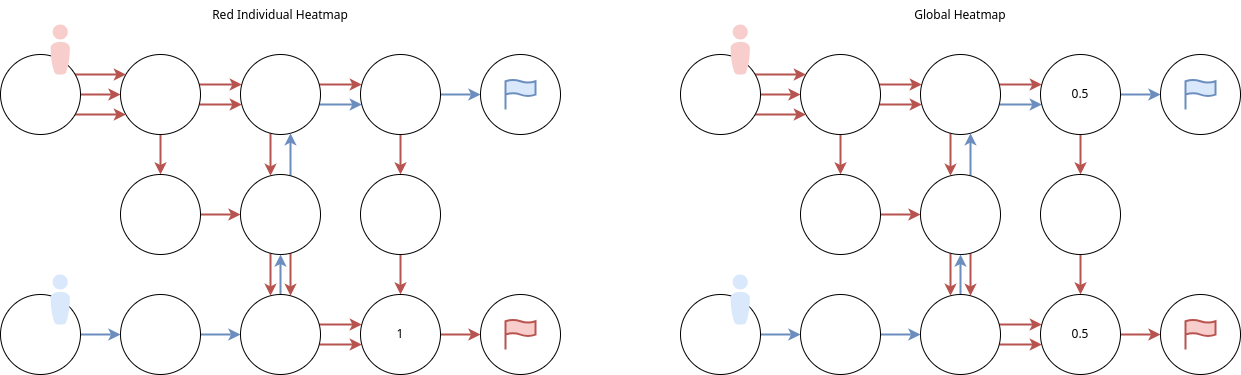
\includegraphics[width=11cm]{img/global_heatmap_p5.drawio.png}
    \end{figure}
\end{frame}



\begin{frame}{Path Elimination Approaches Summary}
    \textbf{Eliminate paths based on heatmaps:}

            \begin{itemize}
                \item \textbf{Unique Heatmap Values:}
                    \begin{itemize}
                        \item Order assignments by global heatmap values.
                        \item Identify critical vertices and eliminate paths containing them.
                    \end{itemize}
                \item \textbf{Threshold-based Elimination:}
                    \begin{itemize}
                        \item Define thresholds (\(\mathcal{H}\)) based on various properties.
                        \item A vertex is denoted critical if its global heatmap value is above the threshold
                    \end{itemize}
                \item \textbf{Sums of Global Heatmap Values:}
                    \begin{itemize}
                        \item For every path, we sum the value of each global heatmap value the paths goes on
                        \item We eliminate \(k\) paths based on the summed value 
                    \end{itemize}
            \end{itemize}
\end{frame}



\begin{frame}{An example}
    \begin{figure}[H]
        \centering
        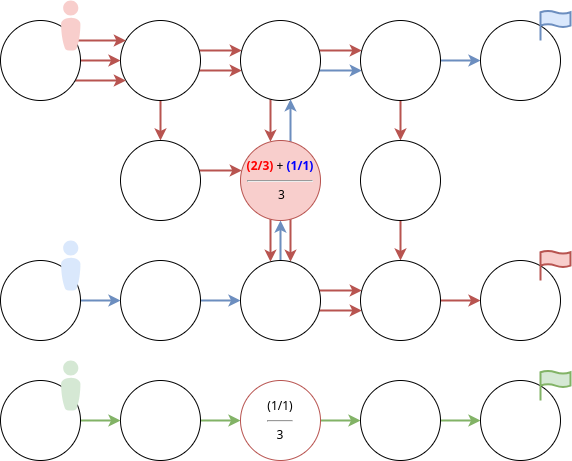
\includegraphics[width=\widthimg]{img/pe_one_heatmap_value_example.drawio.png}
    \end{figure}
\end{frame}





\subsection{Path Selection}
\begin{frame}{Path Selection: towards (partial) solving}
    In the end, what paths are we using? 


    \begin{itemize}
        \item Objective 1: Identify a conflict-free partial plan \(\hat{\Pi}\)
        \begin{itemize}
            \item At most one path per agent 
        \end{itemize}
        \item Objective 2: Create a subgraph 
        \begin{itemize}
            \item At least one path per agent
        \end{itemize}
    \end{itemize}
\end{frame}

\begin{frame}{(Partial) Solving}
    Two solving methods:
    \begin{enumerate}
        \item Using already-computed paths
        \begin{itemize}
            \item Use non-conflicting set of paths as preprocessing for a MAPF algorithm 
        \end{itemize}
        \item Using subgraph
        \begin{itemize}
            \item Using selected paths and using the vertices used by paths to create a subgraph  
        \end{itemize}
    \end{enumerate}
\end{frame}



\begin{frame}{An example}
    \begin{figure}[H]
    \centering
    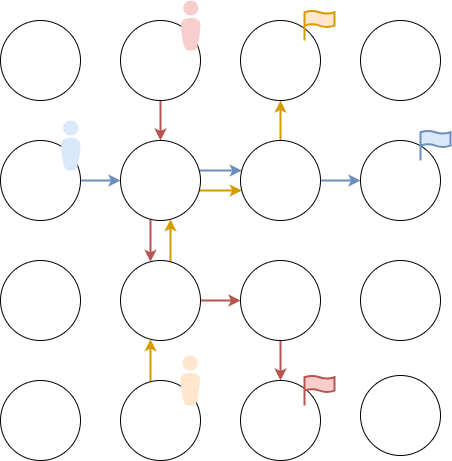
\includegraphics[width=6cm]{img/partial_solving_example.png}
\end{figure}
\end{frame}


\subsection{Pre-computed paths}
\begin{frame}[fragile]{An example using pre-computed paths}
    \begin{figure}[H]
    \centering
    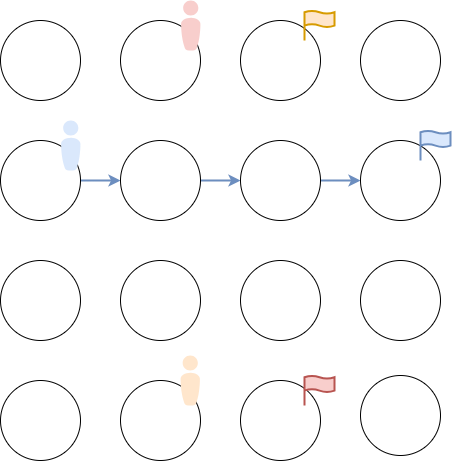
\includegraphics[width=5.5cm]{img/pre_computed_path_solving.drawio.png}
\end{figure}
\end{frame}


\subsection{Subgraph}
\begin{frame}[fragile]{An example using subgraph}
    \begin{figure}[H]
        \centering
        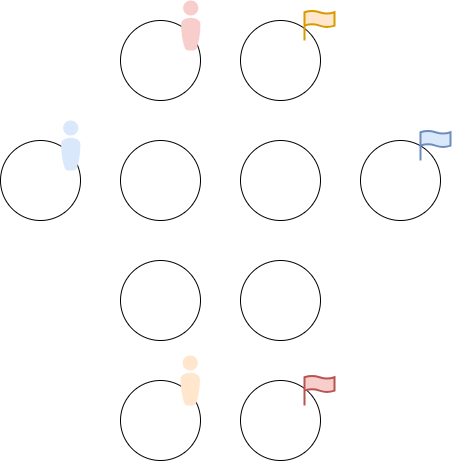
\includegraphics[width=6cm]{img/subgraph_solving.png}
    \end{figure}
\end{frame}

\begin{frame}[fragile]{Subgraph extention strategies}
    
    \begin{figure}[H]
        \centering
        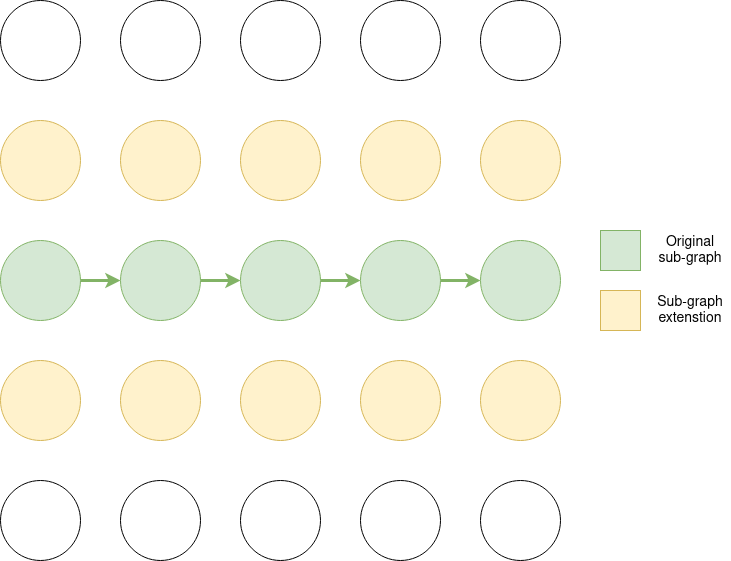
\includegraphics[width=\widthimg]{img/corridor.drawio.png}
    \end{figure}
\end{frame}

\begin{frame}[fragile]{Subgraph extention strategies}
    \begin{figure}[H]
        \centering
        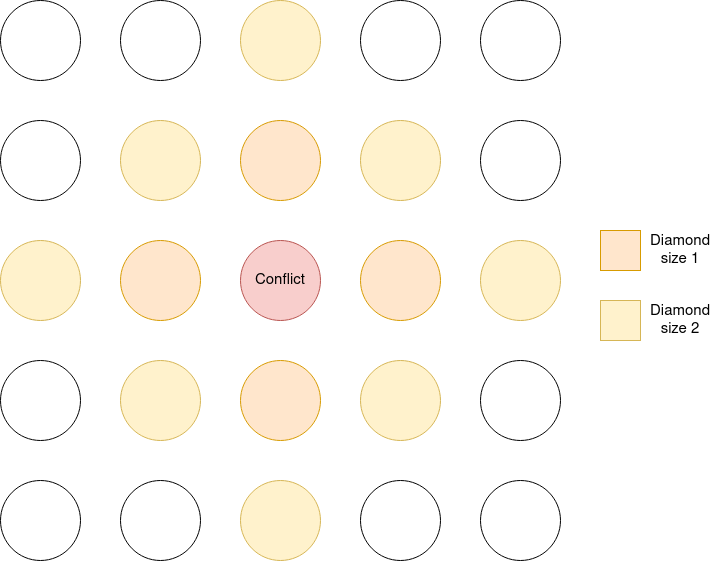
\includegraphics[width=\widthimg]{img/diamond.drawio.png}
      \end{figure}
      
\end{frame}


\section{Benchmarks}
\begin{frame}{Benchmarks}
    We evaluate different approaches against the base MAPF encoding and against a witness approach: 
    
    \(\blacktriangleright\) It consists of one random path per agent converted to a subgraph.

\end{frame}


\begin{frame}{Nomenclature for benchmarks}

    \begin{table}[H]
        \centering
        \label{tbl:nomenclature_approach}
        \begin{tabular}{@{}c|c|c@{}}
        Step Name & Description & Identifier \\ \midrule
        \multirow{2}{*}{IPF} & No Additional path  (15 paths) & \textbf{N} \\
         & Additional Path  (30 paths) & \textbf{A} \\ \midrule
        \multirow{2}{*}{Path Elimination} & Simple threshold & \textbf{St} \\
         & Summed Heatmap & \textbf{Sh} \\ \midrule
        \multirow{2}{*}{\begin{tabular}[c]{@{}c@{}}Solving strategy\end{tabular}} & Pre-computed path & \textbf{Pc} \\
         & Subgraph & \textbf{Sg} \\ \midrule
        \multirow{2}{*}{Subgraph strategy} & Corridor & \textbf{C} \\
         & Diamond & \textbf{D}
        \end{tabular}
    \end{table}
\end{frame}


\begin{frame}{Computation time}
    \tiny
    \begin{table}[H]
\begin{center}
\caption{Approaches: focus on average computation time}
\label{tbl:path_computation_time}
\begin{tabular}{@{}lllllll@{}}
\toprule
 \multicolumn{1}{c}{\multirow{2}{*}{Approach}} & \multirow{2}{*}{\# SAT} & \multicolumn{5}{c}{Average time (in sec)} \\ \cmidrule(l){3-7}  
\multicolumn{1}{c}{} &  & \multicolumn{1}{l|}{Horizon} & 0 & 1 & 3 & 5 \\ \midrule
MAPF & 44 & \cellcolor{lightgrey} & 25.4 & 34.1 & 52.6 & 72.3  \\
Witness & 44 & \cellcolor{lightgrey} & 9.0 & 17.4 & 26.0 & 34.1  \\
NStSgC & 44 & \cellcolor{lightgrey} & 14.7 & 29.4 & 38.0 & 47.0  \\
NShSg & 44 & \cellcolor{lightgrey} & 14.3 & 28.5 & 37.4 & 46.6  \\
NStSg & 44 & \cellcolor{lightgrey} & 14.5 & 29.1 & 37.8 & 46.6  \\
NStSgD & 44 & \cellcolor{lightgrey} & 14.6 & 29.5 & 38.1 & 47.1  \\
NStSgCD & 44 & \cellcolor{lightgrey} & 14.7 & 29.6 & 38.3 & 47.2  \\
\textbf{AShSg} & 44 & \cellcolor{lightgrey} & 16.7 & 29.9 & 38.9 & 48.0  \\
AShSgCD & 44 & \cellcolor{lightgrey} & 17.2 & 30.5 & 39.6 & 48.9  \\
AStSg & 43 & \cellcolor{lightgrey} & 30.9 & 39.5 & 48.5 & 58.0  \\
NStPc & 41 & \cellcolor{lightgrey} & 86.3 & 110.8 & 136.7 & 164.3  \\
NShPc & 41 & \cellcolor{lightgrey} & 101.9 & 114.0 & 141.3 & 170.1  \\
NShSgPcCD & 40 & \cellcolor{lightgrey} & 92.7 & 100.4 & 108.7 & 117.6  \\
AStPc & 39 & \cellcolor{lightgrey} & 128.2 & 152.6 & 178.7 & 206.0  \\
NStSgPc & 38 & \cellcolor{lightgrey} & 131.5 & 138.6 & 146.2 & 154.5  \\
AStSgCD & 37 & \cellcolor{lightgrey} & 153.7 & 161.2 & 169.4 & 177.8  \\
NShSgPc & 37 & \cellcolor{lightgrey} & 152.0 & 159.3 & 167.1 & 175.4  \\
AStSgPc & 37 & \cellcolor{lightgrey} & 153.4 & 160.9 & 169.1 & 177.5  \\
\end{tabular}
\end{center}
\end{table}


\end{frame}

\begin{frame}{Solving proportion}\
    \tiny
    \begin{table}[H]
\begin{center}
\caption{Approaches: focus on solving proportion}
\label{tbl:path_proportion}
\begin{tabular}{@{}lllllll@{}}
\toprule
 \multicolumn{1}{c}{\multirow{2}{*}{Approach}} & \multirow{2}{*}{\# fully solved} & \multicolumn{5}{c}{Expected \% agent with a path} \\ \cmidrule(l){3-7}  
\multicolumn{1}{c}{} &  & \multicolumn{1}{l|}{Horizon} & 0 & 1 & 3 & 5 \\ \midrule
MAPF & 44 & \cellcolor{lightgrey} & 100 & 100 & 100 & 100  \\
\textbf{AShSg} & 39 & \cellcolor{lightgrey} & 97 & 97 & 98 & 98  \\
AShSgCD & 39 & \cellcolor{lightgrey} & 97 & 97 & 98 & 98  \\
Witness & 38 & \cellcolor{lightgrey} & 96 & 97 & 97 & 98  \\
NStSgC & 37 & \cellcolor{lightgrey} & 97 & 97 & 98 & 98  \\
NShSg & 37 & \cellcolor{lightgrey} & 96 & 96 & 97 & 98  \\
AStSg & 37 & \cellcolor{lightgrey} & 97 & 97 & 98 & 98  \\
NStSgD & 37 & \cellcolor{lightgrey} & 97 & 97 & 98 & 98  \\
NStSg & 37 & \cellcolor{lightgrey} & 97 & 97 & 98 & 98  \\
NStSgCD & 37 & \cellcolor{lightgrey} & 97 & 97 & 98 & 98  \\
NShPc & 31 & \cellcolor{lightgrey} & 88 & 89 & 89 & 90  \\
NStPc & 24 & \cellcolor{lightgrey} & 86 & 87 & 88 & 90  \\
NShSgPc & 23 & \cellcolor{lightgrey} & 77 & 78 & 78 & 80  \\
AStPc & 22 & \cellcolor{lightgrey} & 80 & 80 & 82 & 83  \\
NShSgPcCD & 21 & \cellcolor{lightgrey} & 83 & 83 & 84 & 85  \\
AStSgCD & 17 & \cellcolor{lightgrey} & 72 & 72 & 74 & 75  \\
AStSgPc & 17 & \cellcolor{lightgrey} & 72 & 72 & 74 & 75  \\
NStSgPc & 15 & \cellcolor{lightgrey} & 75 & 76 & 77 & 78  \\
\end{tabular}
\end{center}
\end{table}


\end{frame}


\begin{frame}{Detailed performance}
    \tiny
    \begin{table}[]
        \centering
        \caption{Approach Decomposition}\label{tbl:approach_decomposition}
        \begin{tabular}{@{}llllll@{}}
        \toprule
        \multicolumn{1}{l|}{\multirow{2}{*}{Step Name}} & \multicolumn{3}{c|}{Total time} & \multicolumn{2}{c}{\% of the process} \\ \cmidrule(l){2-6}  
        \multicolumn{1}{l|}{} & \multicolumn{1}{l|}{Id.} & \multicolumn{1}{c}{AShSg} & \multicolumn{1}{c|}{Witness} & \multicolumn{1}{c}{AShSg} & Witness \\ \midrule
        IPF & \cellcolor{lightgrey} & 49 & 41  &7\% &10\%  \\
        Heatmaps Computation & \cellcolor{lightgrey} & 14 &  - &2\% & - \\
        Summed Heatmap per Path & \cellcolor{lightgrey} & 0 &  - &0\% & - \\
        Path Elimination & \cellcolor{lightgrey} & 7 &  - &1\% & - \\
        Path Selection & \cellcolor{lightgrey} & 8 & 1  &1\% &0\%  \\
        Partial Solving & \cellcolor{lightgrey} & 551 & 352  &87\% &89\%  \\
        \end{tabular}
        \end{table}
\end{frame}

\section{Conclusion}
\begin{frame}{Conclusion}
\begin{itemize}
    \item Implemented a whole process for Plan merging
    \item Explored different ways of solving
    \item Defined a Plan Merging approach based on heatmaps as a selection process (which can be used for future work)
    \item We showed that some of the approaches we defined can outperform classical MAPF
\end{itemize}
\end{frame}


\begin{frame}{Thanks}
    
    \centering 
    Thank you for your attention !! :) \\[1cm] 
    
    Special thanks to Klaus Strauch, Etienne Tignon, Torsten Schaub \& Lydia Körber 

\end{frame}






\subsection{Input format}
\begin{frame}{Input format}
    \begin{itemize}
        \item \(vertex/1\) 
        \item \(edge/2\)
        \item \(agent/1\) 
        \item \(start/2\) 
        \item \(goal/2\) 
    \end{itemize}
\end{frame}




\subsection{Base Encoding}
\begin{frame}[fragile]{Predicate explanation}
    \begin{itemize}
        \item \(at(R,P,T)\)
        \begin{itemize}
            \item Represent the position of an agent at a specific time step
        \end{itemize}
        \item \(move(R,U,V,T)\)
         \begin{itemize}
            \item Represent the movement of an agent from a vertex to another at a specific time step
        \end{itemize}
    \end{itemize}
\end{frame}




\begin{frame}[fragile]{Base MAPF Encoding}
    \begin{lstlisting}[style=mystyle, caption={Base MAPF Encoding}]
        at(R,P,0) :- start(R,P). 
        time(1..horizon).
    
        {move(R,U,V,T) : edge(U,V)} 1 :- agent(R), time(T). 
    
        at(R,V,T) :- move(R,_,V,T). 
        :- move(R,U,_,T), not at(R,U,T-1). 
        at(R,V,T) :- 
            at(R,V,T-1), 
            not move(R,V,_,T), 
            time(T). 
    
        :- { at(R,V,T) }!=1 , agent(R), time(T). 
    
        :- {at(R,V,T) : agent(R)} > 1, vertex(V), time(T). 
        :- move(_,U,V,T), move(_,V,U,T), U < V. 
            
        :- goal(R,V), not at(R,V,horizon). 
    \end{lstlisting}
\end{frame}


\begin{frame}{MAPF Definition}
    We define MAPF\cite{husvobbass22a} input as such:
        \begin{itemize}
            \item A triple $(V,E,A)$
            \begin{itemize}
                \item $V,E$ a connected graph
                \item $V$ a set of vertices
                \item $E$ a set of edges
                \item $A$ a set of agents
            \end{itemize}
            \item For each agent \(a=(s,g) \in A\), \(s,g \in V\)
        \end{itemize}
\end{frame}


\begin{frame}{MAPF Definition}
    Then, we define output as such:
        \begin{itemize}
            \item The output is a plan \(\Pi\)
            \item \(\Pi\) is a collection of $(\pi_a)_{a\in A}$
            \begin{itemize}
                \item \(\pi_a\) is a finite sequence of vertices in $V$ 
                \item \(\pi_a (t) = v\) 
                \item \(\pi_a(0) = s, \pi_a(|\pi_a|-1) = g, a = (a,g)\)
            \end{itemize}
            \item A plan is valid if no conflict occurs
            \begin{itemize}
                \item Vertex conflict: given any $a,a'\in A$, $\pi_a(t) = \pi_{a'}(t)$
                \item Edge conflict: given any $a,a'\in in A$
                \begin{itemize}
                    \item $\pi_a(t-1) = \pi_{a'}(t)$
                    \item $\pi_a(t) = \pi_{a'}(t-1)$
                \end{itemize}
            \end{itemize}
        \end{itemize}
\end{frame}



\begin{frame}[fragile]{Input format}

    \begin{lstlisting}[style=mystyle]
    agent(1). start(1,(2,1)). goal(1,(2,4)). 
    agent(2). start(2,(2,3)). goal(2,(2,5)).
    agent(3). start(3,(5,4)). goal(3,(1,4)).
    
    vertex((2,3)). vertex((1,4)). vertex((2,4)). vertex((3,4)). vertex((2,2)).
    vertex((4,4)). vertex((2,1)). vertex((5,4)). vertex((2,5)). 
    
    edge((2,4),(1,4)). edge((3,4),(2,4)). edge((2,3),(2,2)). edge((2,4),(2,3)).
    edge((2,5),(2,4)). edge((2,2),(2,1)). edge((2,3),(2,4)). edge((2,4),(2,5)).
    edge((2,1),(2,2)). edge((2,2),(2,3)). edge((1,4),(2,4)). edge((2,4),(3,4)).
    edge((3,4),(4,4)). edge((4,4),(5,4)).
    
    % Optional 
    shortestpath_length(1,3). shortestpath_length(2,2). shortestpath_length(3,4).
    
    makespan(4).
    \end{lstlisting}

\end{frame}


\begin{frame}[fragile]{Base IPF encoding}
    \begin{lstlisting}[style=mystyle, caption={IPF computation}]
        time(1..horizon).

        {at(V,0) : vertex(V)} = 1.
    
        { move(U,V,T) : edge(U,V)} 1 :- time(T).
    
        at(V,T) :- move(_,V,T).
        :- move(U,_,T), not at(U,T-1).
    
        :- { at(V,T) } != 1, time(T).
    
        at(V,T) :- at(V,T-1), not move(V,_,T), time(T).
    
    \end{lstlisting}
\end{frame}



\begin{frame}{Eliminating paths using unique heatmap value}
    \begin{itemize}
        \item Gather all possible assignments of \((v, t)\) within a \(\tau\)
        \item We order then given their associated global heatmap value
        \item We classify vertices with the highest global heatmap value a ``critical''
        \item We then kill (\(n\)) paths having in their sequence the critical vertex identified in the previous step. 
    \end{itemize}
\end{frame}

\begin{frame}{Principle}
    If the Global Heatmap value of a vertex at a specific time point is higher than a defined value \(\mathcal{H}\), the vertex is denoted as critical.
    
    \[
    critical\_vertices(\tau) = \{(v,t) | \Phi(\tau,v,t) > \mathcal{H}, (v,t) \in \mathcal{F}(\tau) \}
    \]

    Thresholds formulas can be defined using any properties.
\end{frame}


\begin{frame}{Simple (Biased) Threshold \& (Biased) Context dependent threshold}
    
    Simple (Biased) Threshold:\\[0.5cm]
    \[
        \mathcal{H}_{sbt}(A,\Delta) =  \frac{1*\Delta}{|A|}
    \]

    \begin{itemize}
        \item Simple equation
        \item Can denote more or less path as ``critical'' using the bias \(\Delta\)
        \item But lacks vertex-specific context
    \end{itemize}
    
    (Biased) Context dependent threshold:\\[0.5cm]
    \[
        \mathcal{H}_{bcdt}(V,T,A,\Delta) = \frac{npath\_on(V,T)*\Delta}{nagent\_on(V,T) * |A|}    
    \]

\end{frame}

\begin{frame}{Eliminating paths using sums of global heatmap values}
    
    Other approaches focus on only one vertex (or few vertices)  at a time.

    \begin{figure}[H]
        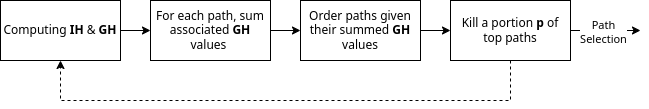
\includegraphics[width=\widthimg]{img/summed_heatmap_value.drawio.png}
    \end{figure}

    \begin{itemize}
        \item Kill Agent quickly if there is not a lot of paths per agents
        \item The more diverse the paths are, the more efficient the approach seems to be
    \end{itemize}

\end{frame}


\begin{frame}[fragile]{Encoding: Towards a partial plan}
    
    \begin{lstlisting}[style=mystyle]
        % Defining collision & possible_path
        possible_path(R,I):- at(R,I,_,_), not path_killed(R,I). |\label{line:possible_path}|
        
        % Constructing a (partial) plan
        {selected_path(R,I) : possible_path(R,I) }1 :-  agent(R). |\label{line:selecting_candidate}|
    
        collision((R1,P1),(R2,P2),T) :- |\label{line:vertex_collision}|
            R1 != R2, at(R1,P1,V,T), at(R2,P2,V,T),
            selected_path(R1,P1), selected_path(R2,P2).
    
        collision((R1,P1),(R2,P2),T) :- |\label{line:edge_collision}|
            R1 != R2, at(R1,P1,V1,T), at(R1,P1,V2,T+1), at(R2,P2,V2,T), 
            at(R2,P2,V1,T+1), selected_path(R1,P1), selected_path(R2,P2).
        
        :- collision((R1,P1),(R2,P2),_), |\label{line:no_collision}|
            selected_path(R1,P1), 
            selected_path(R2,P2).
    
        selected_agent(R) :- selected_path(R,_).  |\label{line:select_agent}|    
    
        #maximize {1@1,R : selected_path(R,_)}. |\label{line:more_agent}|
    \end{lstlisting}
    \end{frame}
    
    
    \begin{frame}[fragile]{Objective: Creating a subgraph}
    \begin{lstlisting}[style=small]
        nvertex(V) :- selected_path(R,I), at(R,I,V,_).
        nedge(U,V) :- 
            edge(U,V), 
            nvertex(U), 
            nvertex(V).
    \end{lstlisting}
    \end{frame}



\begin{frame}[fragile]{(Partial) Solving Encoding}
    We can group the two approaches in one encoding:
    \begin{lstlisting}[style=mystyle, caption={Encoding of final solver}, label={lst:solver}, numbers=left, ,escapechar=|]
    time(1..horizon).

    at(R,P,0) :- start(R,P).

    { move(R,U,V,T) : nedge(U,V)} 1 :- agent(R), time(T).

    at(R,V,T) :- move(R,_,V,T).
            :- move(R,U,_,T), not at(R,U,T-1).

    at(R,V,T) :- 
        at(R,V,T-1), 
        not move(R,V,_,T), 
        time(T).

    :- {at(R,V,T)}!=1, agent(R), time(T).|\label{line:one_position_at_a_time}|

    :- { at(R,V,T) : agent(R) }  > 1, nvertex(V), time(T).
    :- move(_,U,V,T), move(_,V,U,T), U < V.

    goal_reached(R) :- at(R,V,horizon), goal(R,V). |\label{line:ipf_goal_reached}|

    #maximize{1,R : goal_reached(R)}. |\label{line:maximize_goal_reached}|
\end{lstlisting}
\end{frame}



\end{document}
